\documentclass{beamer}%[fleqn,usenatbib]{mnras}
\setbeamertemplate{itemize items}[square]
\mode<presentation>{
\usetheme{Madrid}
}
%\usepackage{cite}
\usepackage{natbib}
\usepackage{enumitem}
\usepackage{setspace}
%\usepackage{enumerate}
\setbeamertemplate{footline}[page number]
\setbeamertemplate{navigation symbols}{}%去掉页面底部的导航符号
%\usepackage{tikz}
\usepackage{amsmath}
\usepackage{mathtools}
\usepackage{booktabs}
%\usepackage[fontset=windows]{ctex}
\usepackage{ctex}
\usepackage{multicol}
\usepackage{setspace}
\usepackage{animate}

%\usefonttheme[onlymath]{serif}
\usefonttheme{serif}
\usepackage{bm}
%\usepackage{algorithm}
\usepackage[ruled]{algorithm2e}
\usepackage{algorithmic}
\usepackage{verbatim}
\usepackage{ulem}
\usepackage{bm}
\usepackage{multicol}
\usepackage{graphicx} %插入图片的包
\usepackage{wrapfig}
\usepackage{subfig}
\usepackage{caption}
\usepackage{multirow}
\titlegraphic{\vspace{0.28\textheight}\flushleft{\hspace{-0.02\textwidth}
\includegraphics[height=0.1\textwidth]{logo.png}}}
\usepackage{ulem}
\newcommand{\revise}[1]{\textcolor[rgb]{1.00,0.00,0.00}{{}#1}}
\newcommand{\reviseok}[1]{\textcolor[rgb]{0.00,0.00,0.00}{{}#1}}
%\newcommand{\proeric}[1]{\textcolor[rgb]{1.00,0.00,1.00}{{}#1}}
\newcommand{\proericok}[1]{\textcolor[rgb]{0.00,0.00,0.00}{{}#1}}
\renewcommand\tablename{表}
\renewcommand\figurename{图}
\renewcommand{\arraystretch}{1.4}
\setbeamertemplate{caption}[numbered]
\usepackage{listings}
\usepackage{xcolor}
\lstset{
    language         = Python,                          %代码语言使用的是python
    frame            = shadowbox,                       %把代码用带有阴影的框圈起来
    rulesepcolor     = \color{red!20!green!20!blue!20}, %代码块边框为淡青色
    keywordstyle     = \color{blue!90}\bfseries,        %代码关键字的颜色为蓝色,粗体
    commentstyle     = \color{red!10!green!70}\textit,  % 设置代码注释的颜色
    showstringspaces = false,                           %不显示代码字符串中间的空格标记
    numbers          = left,                            % 显示行号
    numberstyle      = \tiny,                           % 行号字体
    stringstyle      = \ttfamily,                       % 代码字符串的特殊格式
    breaklines       = true,                            %对过长的代码自动换行
    extendedchars    = false,                           %解决代码跨页时,章节标题,页眉等汉字不显示的问题
    %escapebegin     = \begin{CJK*},                    escapeend = \end{CJK*}, % 代码中出现中文必须加上,否则报错
    texcl            = true,
    escapeinside     = ``,
    xleftmargin      = 1em,
    xrightmargin     = 1em,
    aboveskip        = 1em
}

\def\IDM{IDM}
\def\PR{PR}

\title[目标检测]{目标检测}
%\tiny \scriptsize \footnotesize \small \normalsize \large \Large \LARGE \huge \Huge
\author{\large 李乡儒} %{\scriptsize Email: xiangru.li@qq.com}}
\institute[SCNU]{\small
华南师范大学计算机学院
%国家气象中心
}
\date{\today}
%\data{2020年11月26日}

\begin{document}
\graphicspath{{figures/}}

\begin{frame}%[plain]          %“帧”的开始(帧即是一页幻灯片)
    \titlepage
    %\vspace{-2cm}
    %{\setlength{\baselineskip}{-6pt}
    %{\noindent \tiny{Qingguo Zeng, Xue Chen, Xiangru Li*, Jinlin Han, Chen Wang, Dejiang Zhou, Tao Wang.  Radio Frequency Interference Mitigation based on ArPLS and SumThreshold. Monthly Notices of the Royal Astronomical Society ,Volume 500, Issue 3, January 2021, Pages 2969–2978.}}}
\end{frame}

\begin{frame}[allowframebreaks]
    \frametitle{\textsc{目录}} \vspace{-0.3cm}
    \begin{spacing}{0.0}
        \tableofcontents[hideallsubsections]
    \end{spacing}   % 若不想要目录, 注释掉该句
\end{frame}

\begin{frame}[allowframebreaks]
    \vspace{-0.2cm}
    {\noindent\large\textbf{内容概要}}
    \vspace{0.4cm}
    \begin{itemize}
        \item[$ \bullet $] 什么是目标检测
        \item[$ \bullet $] 如何表示
        \item[$ \bullet $] 基础知识
        \item[$ \bullet $] Fast RCNN
        \item[$ \bullet $] YOLO
    \end{itemize}

\end{frame}

\section{什么是目标检测}

\begin{frame}[allowframebreaks]
    \frametitle{\textsc{目录}} \vspace{-0.3cm}
    \begin{spacing}{0.0}
        \tableofcontents[currentsection,hideallsubsections]
    \end{spacing}   % 若不想要目录, 注释掉该句
\end{frame}



\begin{frame}
    \noindent\large\textbf{目标检测}
    \vspace{0.4cm}
    \begin{itemize}
        \item[$ \bullet $] 是什么?
        \item[$ \bullet $] 在哪里?
        \item[$ \bullet $] 有哪些?
    \end{itemize}
    \vspace{1cm}
    “是什么”意味着需要判断出找出来的目标是什么,也就是对目标的类别做判断,是人还是狗或者是车\\
    \vspace{1em}
    “在哪里”需要指出找到的目标在图像的那个地方,范围是哪里\\
    \vspace{1em}
    “有哪些”意味着需要将图像当中所有的感兴趣物体(预先定义的类别)找出来\\
\end{frame}

\begin{frame}
    \noindent\large\textbf{如何表示}\\
    在计算机当中需要用数字来表达“是什么”、“在哪里”、“在哪里”
    \vspace{1em}
    \begin{itemize}
        \item[$ \bullet $] 整数(one-hot 向量)表示类别
        \item[$ \bullet $] 矩形框表示位置(四元组$[x,y,w,h]$)
        \item[$ \bullet $] 堆叠所有目标组成数组$n\times5$
    \end{itemize}
    \vspace{1em}
    \begin{figure}
        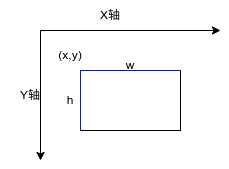
\includegraphics[width=0.3\linewidth]{box.png}
    \end{figure}
\end{frame}

\begin{frame}
    \noindent\large\textbf{基础知识}
    \begin{itemize}
        \item[$ \bullet $] 矩形框的3种表示
            矩形框的表示形式有:\\
            $[x,y,w,h]$ \\
            $[x_1,y_1,x_2,y_2]([left,top,right,bottom])$\\
            $[cx,cy,w,h]$
        \item[$ \bullet $] 交并比(IoU)
            交并比是指两个矩形的交集与并集的面积之比$IoU=\frac{|A\cap B|}{|A\cup B|}$,
            实现是采用第二种矩形表示进行实现$A[l_A,t_A,r_A,b_A],B[l_B,t_B,r_B,b_B]$:\\

            $S_A=(r_A-l_A)\times(b_A-t_A)$\\
            $S_B=(r_B-l_B)\times(b_B-t_B)$\\
            $W_{AB}=(min(r_A,r_B)-max(l_A,l_B))$\\
            $H_{AB}=(min(b_A,b_B)-max(t_A,t_B))$\\
            if $ W_{AB}<0$ or $H_{AB}<0$ then $IoU = 0$\\
            else $IoU=\frac{W_{AB}\times H_{AB}}{S_A+S_B-W_{AB}\times H_{AB}}$

    \end{itemize}
\end{frame}


\begin{frame}
    \noindent\large\textbf{常见数据集}

    %    \begin{itemize}
    %    \item[$ \bullet $]  包含图像和标签(掩码、mask、Ground Truth)
    %
    %    %\vspace{1em}
    %    \item[$ \bullet $]  图像与标签大小相同
    %
    %    %\vspace{1em}
    %    \item[$ \bullet $]  图像与标签的像素一一对应
    %
    %    %\vspace{1em}
    %    \item[$ \bullet $] 标签的形式多种多样,包括图像、描述文件、表格等形式
    %    \end{itemize}
    %
    %    \vspace{1em}
    %    \noindent\large\textbf{常见数据集}

    \vspace{1em} \small
    Common Objects in COntext(COCO)、PASCAL Visual Object Classes(PASAL)、
    The Cityscapes Dataset、The Cambridge-driving Labeled Video Database(CamVid)、
    Stanford Background Dataset、Barcelona Dataset、Microsoft Research in Cambridge、
    LITS Liver Tumor Segmentation Dataset、ISBI Challenge
\end{frame}



\begin{frame}
    \noindent\large\textbf{常用评价指标}

    \vspace{0.1em}
    $\bullet$ 准确率:$PA=\frac{TP+TN}{TP+FP+FN+TN}$

    \vspace{0.1em}
    $\bullet$ Dice系数(Dice score, F1分数):$dice(A,B)=\frac{2|A\cap B|}{|A|+|B|}=\frac{2TP}{2TP+FN+FP}$

    \vspace{0.1em}
    $\bullet$ 雅卡尔指数(交并比):$IoU=\frac{|A\cap B|}{|A \cup B|} = \frac{TP}{TP + FN + FP}$

    \vspace{0.1em}
    $IoU= \frac{Dice}{2-Dice}$; A: 目标像素的集合;B: 算法判定为目标像素的集合。除此之外还有精确率、召回率、平均准确率、平均精确率、平均召回率和聚合雅卡尔指数等指标

    \begin{figure}
        \subfloat[TP、FP、FN]{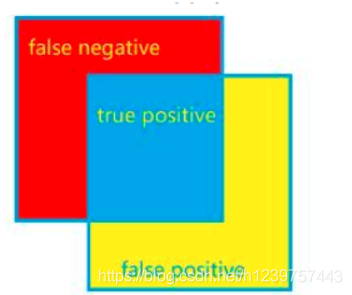
\includegraphics[width=0.3\linewidth]{TPFPFN.png}}
        \subfloat[IoU与Dice]{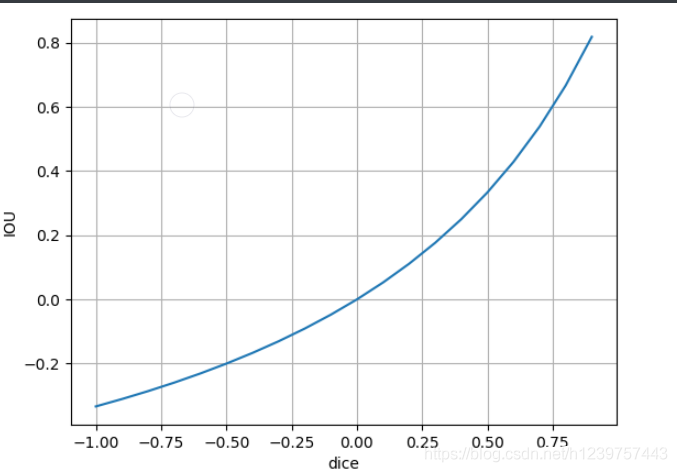
\includegraphics[width=0.3\linewidth]{IoUDice.png}}
    \end{figure}

\end{frame}

\begin{frame}
    \noindent\large\textbf{类别不平衡问题}

    \vspace{1em}
    图像当中的背景与前景常存在像素点数量不平衡的问题,这容易导致模型将所有像素点预测为同一个类别
    \begin{figure}
        
\includegraphics[width=8.0cm]{11.png}
    \end{figure}
\end{frame}

\begin{frame}
    \noindent\large\textbf{解决方法}

    \vspace{1em}
    $\bullet$ 损失函数加权:$L=\sum w_iloss_i$

    \vspace{1em}
    $\bullet$ 欠采样:样本多的类别只统计一部分像素点的损失

    \vspace{1em}
    $\bullet$ Dice损失函数:$L=1-\frac{2\sum \hat{y}_iy_i+\epsilon}{\sum (\hat{y}_i+y_i)+\epsilon}$

    \vspace{1em}
    $\bullet$ Focal损失函数:$L=-\sum (1-\hat{y}_i)^\gamma log(\hat{y}_i)$


\end{frame}

\begin{frame}
    \noindent\large\textbf{图像分割的应用}

    \vspace{1em}
    $\bullet$ 自动驾驶:对周围环境图像进行分割

    \vspace{1em}
    $\bullet$ 医学图像病灶检测:将医学影像当中的病变部位分割出来

    \vspace{1em}
    $\bullet$ 零售图像识别:对货架商品进行监控

    \vspace{1em}
    $\bullet$ 人脸识别:从图像当中提取人脸区域
\end{frame}


\section{U-net:模型与原理}
\begin{frame}[allowframebreaks]
  \frametitle{\textsc{目录}} \vspace{-0.3cm}
    \begin{spacing}{0.0}
        \tableofcontents[currentsection,hideallsubsections]
    \end{spacing}   % 若不想要目录, 注释掉该句
\end{frame}



\begin{frame}
    \noindent\large\textbf{U-net}

    \vspace{1em}
    U-net首次提出是在2015年的MICCAI会议上,此后成为了图像分割任务的baseline,
    主流的图像分割模型大多遵循U-net的基本框架。

    \begin{figure}
        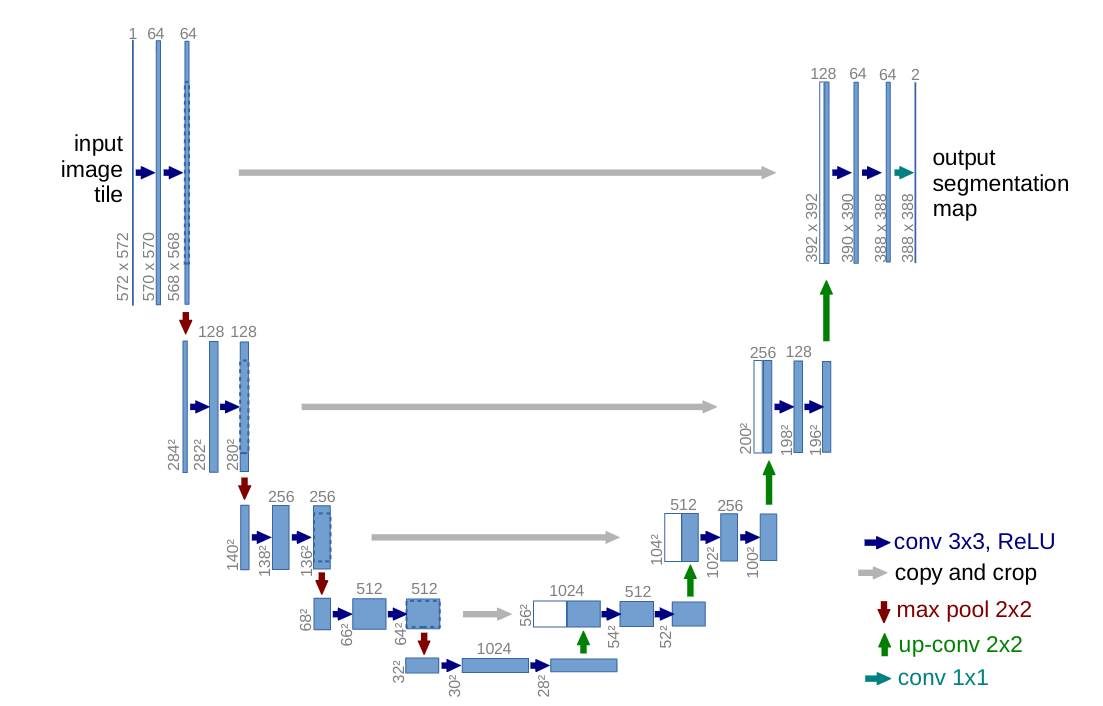
\includegraphics[width=9.5cm]{6.png}
    \end{figure}
\end{frame}

\begin{frame}
    \noindent\large\textbf{无缝分割策略}

    \vspace{1em}
    %U-net首次提出是在2015年的MICCAI会议上,此后成为了图像分割任务的baseline,
    %主流的图像分割模型大多遵循U-net的基本框架。

    \begin{figure}
        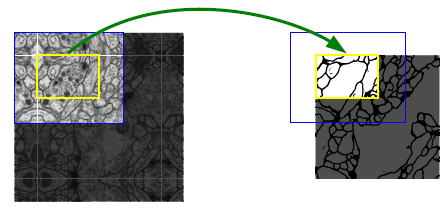
\includegraphics[width=9.5cm]{overlapTile.png}
    \end{figure}
\end{frame}

\begin{frame}
    \noindent\large\textbf{处理流程}

    \vspace{1em}
    \begin{figure}
        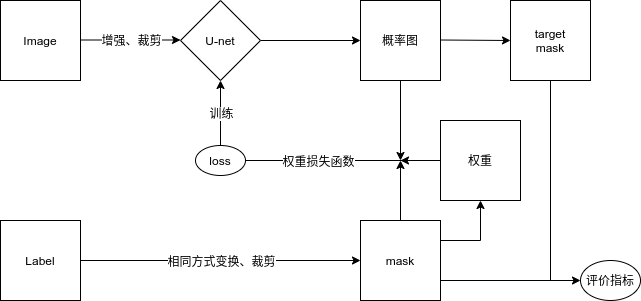
\includegraphics[width=10cm]{10.png}
    \end{figure}
\end{frame}

\begin{frame}
    \noindent\large\textbf{U-net为什么有效}

    \vspace{1em}
    $\bullet$ 跳跃连接保留了更多细节

    \vspace{1em}
    $\bullet$ 多层次特征图能够学习语义特征

    \vspace{1em}
    $\bullet$ 多层次特征融合既能保留细节又能学习语义

    \begin{figure}
        \centering
        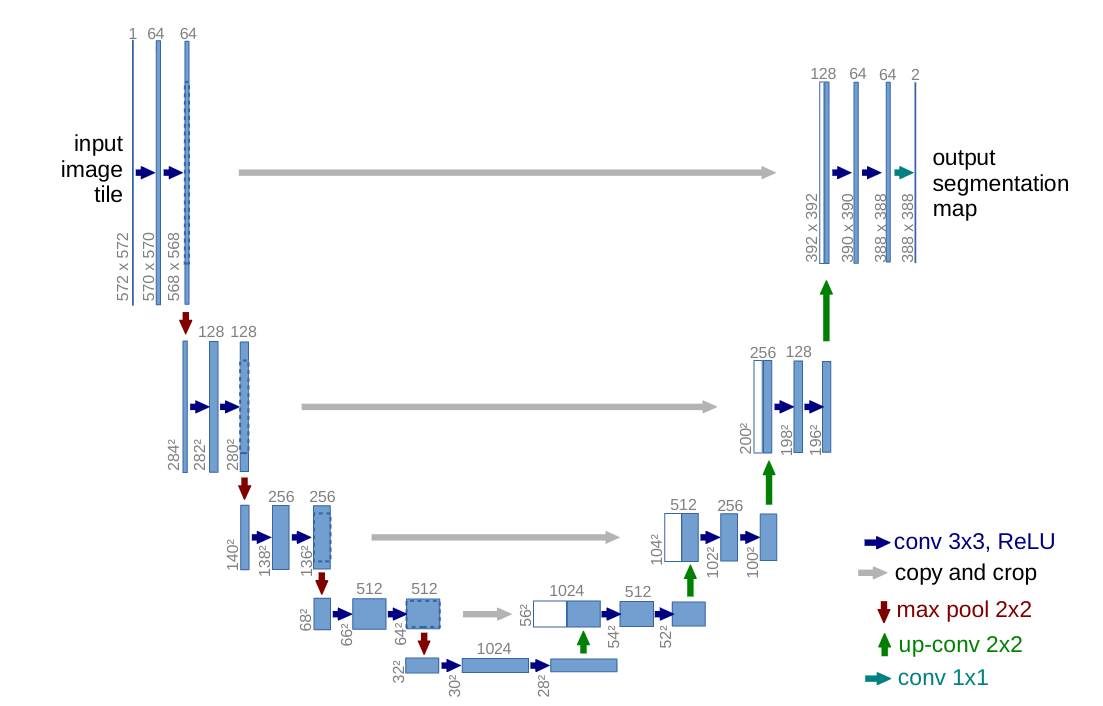
\includegraphics[height=5cm]{6.png}
    \end{figure}


\end{frame}

\begin{frame}
    \noindent\large\textbf{上采样方法}
    \vspace{1em}

    $\bullet$ 采样(线性插值、三次插值、最临近等)

    \begin{figure}
        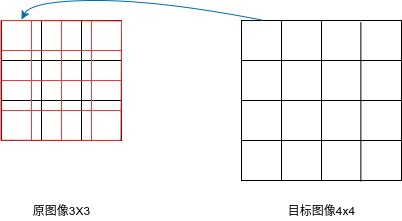
\includegraphics[width=8cm]{8.png}
    \end{figure}

    $\bullet$ 转置卷积(反卷积)
    \begin{figure}
        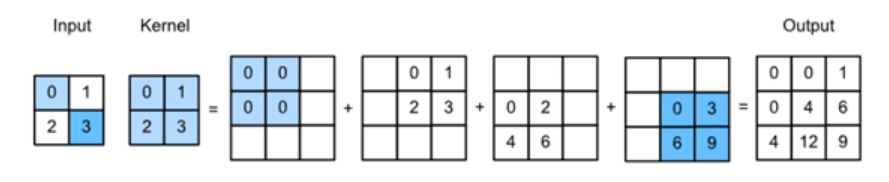
\includegraphics[width=11cm]{7.png}
    \end{figure}

\end{frame}

\begin{frame}
    $\bullet$ 上池化

    \begin{figure}
        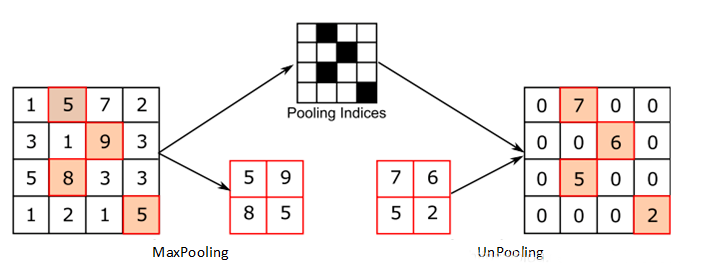
\includegraphics[width=11cm]{9.png}
    \end{figure}

    \vspace{1em}
    在pytorch的MaxPool操作当中,可以选择输出选取的位置,
    而MaxUnPool操作需要特征图和位置作为输入
\end{frame}

\begin{frame}[fragile]
    \begin{lstlisting}
# 采样
torch.nn.functional.interpolate()
torch.nn.functional.grid_sample()
torch.nn.functional.upsample()
torch.nn.UpsamplingBilinear2d
torch.nn.UpsamplingNearest2d
torch.nn.Upsample
# 转置卷积(反卷积)
torch.nn.ConvTranspose2d
torch.nn.functional.conv_transpose2d()
# 上池化
torch.nn.MaxUnpool2d
torch.nn.functional.max_unpool2d()
    \end{lstlisting}
\end{frame}

\begin{frame}

    \vspace{-5em}
    \noindent\large\textbf{特征图融合方法}


    \normalsize
    \vspace{1em}
    $\bullet$ 拼接:在通道维度上将特征图拼接起来

    \vspace{1em}
    $\bullet$ 相加:把相同形状的特征图直接相加

    \vspace{1em}
    区别:拼接不需要通道数一致但需要图尺寸相同,而相加需\\
    \quad \quad \quad 要通道数和图尺寸保持一致

    \vspace{1em}
    联系:相加可以看作是特殊的拼接,因为通常在拼接后会使用\\
    \quad \quad \quad$1\times1$卷积进行加权

\end{frame}

\begin{frame}
    \noindent\large\textbf{特征图融合方法}

    \vspace{1em}
    U-net首次提出是在2015年的MICCAI会议上,此后成为了图像分割任务的baseline,
    主流的图像分割模型大多遵循U-net的基本框架。

    \begin{figure}
        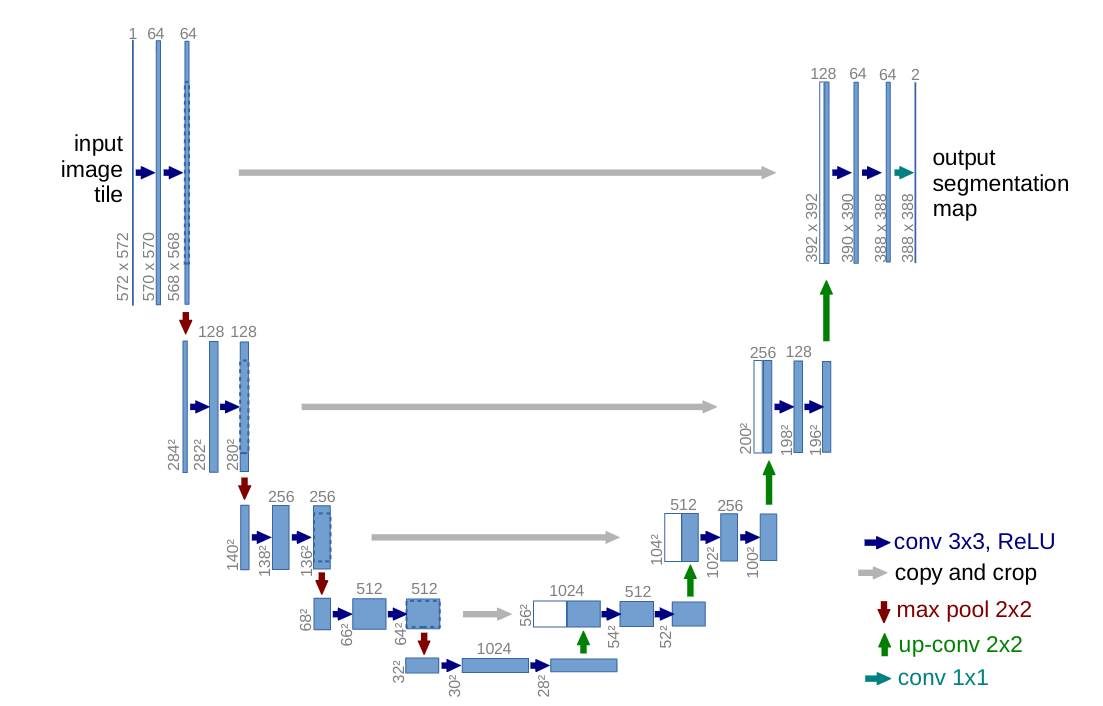
\includegraphics[width=9.5cm]{6.png}
    \end{figure}
\end{frame}


\section{目标检测方法}

\begin{frame}[allowframebreaks]
    \frametitle{\textsc{目录}} \vspace{-0.3cm}
    \begin{spacing}{0.0}
        \tableofcontents[currentsection,hideallsubsections]
    \end{spacing}   % 若不想要目录, 注释掉该句
\end{frame}

\begin{frame}
    目标检测有两个主要流派:Anchor-based与Anchor-Free,两类算法的主要区别在于算法当中是否有预设锚框\\
    \begin{itemize}
        \item[$ \bullet $] Anchor-based:YOLOv3、SSD、Faster \;R-CNN
        \item[$ \bullet $] Anchor-Free:YOLOv1、CornerNet、CenterNet、FCOS
    \end{itemize}

    \vspace{1em}
    另外一个划分是:一阶段和二阶段算法,阶段主要是指从输入到结果之间网络模型的运算次数\\
    \begin{itemize}
        \item[$ \bullet $] 一阶段:YOLO、SSD、CornerNet、CenterNet、FCOS
        \item[$ \bullet $] 二阶段:R-CNN、Faster \;R-CNN
    \end{itemize}

    \vspace{1em}
    在后面的算法当中将介绍二阶段Anchor-based算法Faster\; R-CNN和一阶段Anchor-Free算法YOLOv1\\

\end{frame}


\begin{frame}
    \noindent\large\textbf{基础知识}
    \begin{itemize}
        \item[$ \bullet $] 矩形框的3种表示
            矩形框的表示形式有:\\
            $[x,y,w,h]$ \\
            $[x_1,y_1,x_2,y_2]([left,top,right,bottom])$\\
            $[cx,cy,w,h]$
        \item[$ \bullet $] 交并比(IoU)
            交并比是指两个矩形的交集与并集的面积之比$IoU=\frac{|A\cap B|}{|A\cup B|}$,
            实现是采用第二种矩形表示进行实现$A[l_A,t_A,r_A,b_A],B[l_B,t_B,r_B,b_B]$:\\
            $S_A=(r_A-l_A)\times(b_A-t_A)$\\
            $S_B=(r_B-l_B)\times(b_B-t_B)$\\
            $W_{AB}=(min(r_A,r_B)-max(l_A,l_B))$\\
            $H_{AB}=(min(b_A,b_B)-max(t_A,t_B))$\\
            if $ W_{AB}<0$ or $H_{AB}<0$ then $IoU = 0$\\
            else $IoU=\frac{W_{AB}\times H_{AB}}{S_A+S_B-W_{AB}\times H_{AB}}$
            % \hspace{10cm}
            \vspace{-3.5cm}
            \begin{figure}
                \hspace{6cm}
                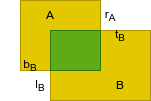
\includegraphics[width=0.4\linewidth]{iou.png}
            \end{figure}
    \end{itemize}
\end{frame}

% \begin{frame}
%     \large
%     \textcolor{vscodedef}{def}  \textcolor{vscodefuncation}{boxIou}\textcolor{vscodebracket}{(}\textcolor{vscodeparameter}{boxes1}: \textcolor{vscodeclass}{Tensor}, \textcolor{vscodeparameter}{boxes2}: \textcolor{vscodeclass}{Tensor}\textcolor{vscodebracket}{)}->\textcolor{vscodeclass}{Tensor}:\\
%     \vspace{0.2em}
%     \qquad\textcolor{vscodecomment}{\# boxes1:(N,4) boxes2:(M,4) use 'xyxy'}\\
%     \vspace{0.2em}
%     \qquad\textcolor{vscodeparameter}{area1}=\textcolor{vscodebracket}{(}\textcolor{vscodeparameter}{boxes1}\textcolor{vscodecomment}{[}:,\textcolor{vscodecomment}{2]}-\textcolor{vscodeparameter}{boxes1}\textcolor{vscodecomment}{[}:,\textcolor{vscodecomment}{0]}\textcolor{vscodebracket}{)}*\textcolor{vscodebracket}{(}\textcolor{vscodeparameter}{boxes1}\textcolor{vscodecomment}{[}:,\textcolor{vscodecomment}{3]}-\textcolor{vscodeparameter}{boxes1}\textcolor{vscodecomment}{[}:,\textcolor{vscodecomment}{1]}\textcolor{vscodebracket}{)}\\
%     \vspace{0.2em}
%     \qquad\textcolor{vscodeparameter}{area2}=\textcolor{vscodebracket}{(}\textcolor{vscodeparameter}{boxes1}\textcolor{vscodecomment}{[}:,\textcolor{vscodecomment}{2]}-\textcolor{vscodeparameter}{boxes2}\textcolor{vscodecomment}{[}:,\textcolor{vscodecomment}{0]}\textcolor{vscodebracket}{)}*\textcolor{vscodebracket}{(}\textcolor{vscodeparameter}{boxes1}\textcolor{vscodecomment}{[}:,\textcolor{vscodecomment}{3]}-\textcolor{vscodeparameter}{boxes2}\textcolor{vscodecomment}{[}:,\textcolor{vscodecomment}{1]}\textcolor{vscodebracket}{)}\\
%     \vspace{0.2em}
%     \qquad\textcolor{vscodeparameter}{lt}=\textcolor{vscodeclass}{torch}.\textcolor{vscodefuncation}{max}\textcolor{vscodebracket}{(}\textcolor{vscodeparameter}{boxes1}\textcolor{vscodecomment}{[}:,\textcolor{vscodedef}{None},:\textcolor{vscodecomment}{2]},\textcolor{vscodeparameter}{boxes2}\textcolor{vscodecomment}{[}:,:\textcolor{vscodecomment}{2]}\textcolor{vscodebracket}{)}  \textcolor{vscodecomment}{\# [N,M,2]}\\
%     \vspace{0.2em}
%     \qquad\textcolor{vscodeparameter}{rb}=\textcolor{vscodeclass}{torch}.\textcolor{vscodefuncation}{min}\textcolor{vscodebracket}{(}\textcolor{vscodeparameter}{boxes1}\textcolor{vscodecomment}{[}:,\textcolor{vscodedef}{None},\textcolor{vscodecomment}{2}:\textcolor{vscodecomment}{]},\textcolor{vscodeparameter}{boxes2}\textcolor{vscodecomment}{[}:,\textcolor{vscodecomment}{2}:\textcolor{vscodecomment}{]}\textcolor{vscodebracket}{)}  \textcolor{vscodecomment}{\# [N,M,2]}\\
%     \vspace{0.2em}
%     \qquad\textcolor{vscodeparameter}{wh}=\textcolor{vscodebracket}{(}\textcolor{vscodeparameter}{rb}-\textcolor{vscodeparameter}{lt}\textcolor{vscodebracket}{)}.\textcolor{vscodefuncation}{clamp}
%     \textcolor{vscodebracket}{(}\textcolor{vscodeparameter}{min}=\textcolor{vscodecomment}{0}\textcolor{vscodebracket}{)}\\
%     \vspace{0.2em}
%     \qquad\textcolor{vscodeparameter}{inter}=\textcolor{vscodeparameter}{wh}\textcolor{vscodebracket}{[}...,\textcolor{vscodecomment}{0}\textcolor{vscodebracket}{]}*\textcolor{vscodeparameter}{wh}\textcolor{vscodebracket}{[}...,\textcolor{vscodecomment}{1}\textcolor{vscodebracket}{]}  \textcolor{vscodecomment}{\# [N,M]}\\
%     \vspace{0.2em}
%     \qquad\textcolor{vscodeparameter}{union}=\textcolor{vscodeparameter}{area1}\textcolor{vscodebracket}{[}:,\textcolor{vscodedef}{None}\textcolor{vscodebracket}{]}+\textcolor{vscodeparameter}{area2}-\textcolor{vscodeparameter}{inter}\\
%     \vspace{0.2em}
%     \qquad\textcolor{vscodereturn}{return} \textcolor{vscodeparameter}{inter}/\textcolor{vscodeparameter}{union}
% \end{frame}

\begin{frame}
    \vspace{1em}
    \noindent\large\textbf{矩形框resize}\\
    \vspace{1em}
    在实际操作当中需要对输入的图像进行resize操作,但是这会导致矩形框的偏移,因此需要对矩形框进行相应变化\\
    \begin{figure}
        \subfloat[源图像]{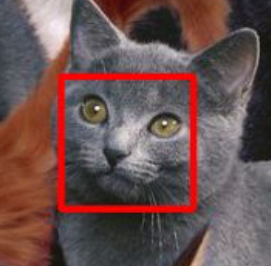
\includegraphics[width=3.3cm,height=3.3cm]{uTools_1651134324913.png}}
        \hspace{1cm}
        \subfloat[目标图像]{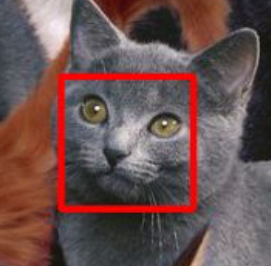
\includegraphics[width=2.4cm,height=1.5cm]{uTools_1651134324913.png}}
    \end{figure}
    图像宽高改变后,坐标点$(x,y)$和矩形框的宽高$(w,h)$按比例变化,源宽高为$(w_o,h_o)$,目标宽高为$(w_t,h_t)$:
    $$x'=\frac{xw_t}{w_o},y'=\frac{yh_t}{h_o}$$
\end{frame}

% \begin{frame}
%     \large
%     @\textcolor{vscodeclass}{no\_grad}\textcolor{vscodebracket}{()}\\
%     \vspace{0.2em}
%     \textcolor{vscodedef}{def} \textcolor{vscodefuncation}{resizeBox}\textcolor{vscodebracket}{(}\\
%     \vspace{0.2em}
%     \qquad\textcolor{vscodeparameter}{orgsize}:\textcolor{vscodeclass}{Tuple}\textcolor{vscodecomment}{[}\textcolor{vscodeclass}{int},\textcolor{vscodeclass}{int}\textcolor{vscodecomment}{]},\\
%     \vspace{0.2em}
%     \qquad\textcolor{vscodeparameter}{tarsize}:\textcolor{vscodeclass}{Tuple}\textcolor{vscodecomment}{[}\textcolor{vscodeclass}{int},\textcolor{vscodeclass}{int}\textcolor{vscodecomment}{]},\\
%     \vspace{0.2em}
%     \qquad\textcolor{vscodeparameter}{boxes}:\textcolor{vscodeclass}{Tensor}\\
%     \vspace{0.2em}
%     \qquad\textcolor{vscodebracket}{)}->\textcolor{vscodeclass}{Tensor}:\\
%     \vspace{0.2em}
%     \qquad\textcolor{vscodeparameter}{orgsize},\textcolor{vscodeparameter}{tarsize}=\textcolor{vscodeclass}{Tensor}\textcolor{vscodebracket}{(}\textcolor{vscodeparameter}{orgsize}\textcolor{vscodebracket}{)},\textcolor{vscodeclass}{Tensor}\textcolor{vscodebracket}{(}\textcolor{vscodeparameter}{tarsize}\textcolor{vscodebracket}{)}\\
%     \vspace{0.2em}
%     \qquad\textcolor{vscodeparameter}{matrix}=\textcolor{vscodeclass}{torch}.\textcolor{vscodefuncation}{diag}\textcolor{vscodebracket}{(}\textcolor{vscodeparameter}{tarsize}/\textcolor{vscodeparameter}{orgsize}\textcolor{vscodebracket}{)}\\
%     \vspace{0.2em}
%     \qquad \textcolor{vscodereturn}{return} \textcolor{vscodeclass}{torch}.\textcolor{vscodefuncation}{cat}\textcolor{vscodebracket}{(}\textcolor{vscodecomment}{[}\textcolor{vscodeparameter}{boxes}\textcolor{vscode3bracket}{[}:,:\textcolor{vscodecomment}{2}\textcolor{vscode3bracket}{]}@\textcolor{vscodeparameter}{matrix},\textcolor{vscodeparameter}{boxes}\textcolor{vscode3bracket}{[}:,:\textcolor{vscodecomment}{2}\textcolor{vscode3bracket}{]}@\textcolor{vscodeparameter}{matrix}\textcolor{vscodecomment}{]},-\textcolor{vscodecomment}{1}\textcolor{vscodebracket}{)}
% \end{frame}



\begin{frame}
    \vspace{0.5em}
    \noindent\large\textbf{非极大值抑制}\\
    \vspace{0.5em}
    非极大值抑制(NMS)主要用来去除重复的预测框,其输入是预测框数组与对应的置信度数组,算法过程如下:\\
    \vspace{0.5em}
    按置信的从大到小排序\\
    While 数组非空:\\
    \qquad 取出置信度最大的预测框 B\\
    \qquad B放入结果集\\
    \qquad 对于剩余数组当中每一个预测框b:\\
    \qquad \qquad if IoU(B,b)>阈值:\\
    \qquad \qquad \qquad 从数组中删除b\\

    \begin{figure}
        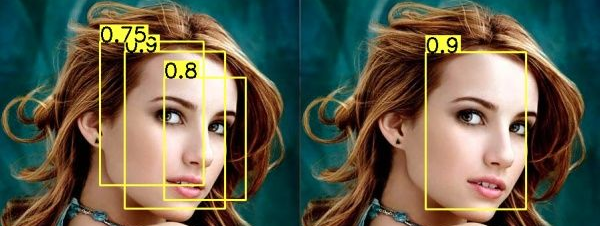
\includegraphics[width=0.7\linewidth]{NMS.png}
    \end{figure}

\end{frame}

% \begin{frame}
%     \large
%     @\textcolor{vscodeclass}{no\_grad}\textcolor{vscodebracket}{()}\\
%     \vspace{0.2em}
%     \textcolor{vscodedef}{def}  \textcolor{vscodefuncation}{nms}\textcolor{vscodebracket}{(}\textcolor{vscodeparameter}{boxes}:\textcolor{vscodeclass}{Tensor},\textcolor{vscodeparameter}{score}:\textcolor{vscodeclass}{Tensor}, \textcolor{vscodeparameter}{threshold}:\textcolor{vscodeclass}{float}\textcolor{vscodebracket}{)}->\textcolor{vscodeclass}{Tensor}:\\
%     \vspace{0.2em}
%     \qquad\textcolor{vscodecomment}{\# boxes:(N,4) score:(N)}\\
%     \vspace{0.2em}
%     \qquad\textcolor{vscodeparameter}{\_},\textcolor{vscodeparameter}{indexes}=\textcolor{vscodeparameter}{score}.\textcolor{vscodefuncation}{sort}\textcolor{vscodebracket}{(}\textcolor{vscodeparameter}{descending}=\textcolor{vscodedef}{True}\textcolor{vscodebracket}{)}\\
%     \vspace{0.2em}
%     \qquad\textcolor{vscodeparameter}{result}=\textcolor{vscodebracket}{[]}\\
%     \vspace{0.2em}
%     \qquad\textcolor{vscodereturn}{while} \textcolor{vscodecomment}{0} \textcolor{vscodedef}{not in }\textcolor{vscodeparameter}{indexes}.\textcolor{vscodeparameter}{shape}:\\
%     \vspace{0.2em}
%     \qquad\qquad\textcolor{vscodeparameter}{result}.\textcolor{vscodefuncation}{append}\textcolor{vscodebracket}{(}\textcolor{vscodeparameter}{indexes}\textcolor{vscodecomment}{[0]}\textcolor{vscodebracket}{)}\\
%     \vspace{0.2em}
%     \qquad\qquad\textcolor{vscodeparameter}{temp\_boxes}=\textcolor{vscodeparameter}{boxes}\textcolor{vscodecomment}{[}\textcolor{vscodeparameter}{indexes}\textcolor{vscodecomment}{]}\\
%     \vspace{0.2em}
%     \qquad\qquad\textcolor{vscodeparameter}{ious}=\textcolor{vscodefuncation}{boxIou}\textcolor{vscodebracket}{(}\textcolor{vscodeparameter}{temp\_boxes}\textcolor{vscodecomment}{[}:\textcolor{vscodecomment}{1]},\textcolor{vscodeparameter}{temp\_boxes}\textcolor{vscodecomment}{[1}:\textcolor{vscodecomment}{]}\textcolor{vscodebracket}{)[}\textcolor{vscodecomment}{0}\textcolor{vscodebracket}{]}\\
%     \vspace{0.2em}
%     \qquad\qquad\textcolor{vscodeparameter}{indexes}=\textcolor{vscodeparameter}{indexes}\textcolor{vscodebracket}{[}\textcolor{vscodecomment}{1}:\textcolor{vscodebracket}{][}\textcolor{vscodeparameter}{ious}<=\textcolor{vscodeparameter}{threshold}\textcolor{vscodebracket}{]}\\
%     \vspace{0.2em}
%     \qquad\textcolor{vscodereturn}{return} \textcolor{vscodeclass}{torch}.\textcolor{vscodefuncation}{stack}\textcolor{vscodebracket}{(}\textcolor{vscodeparameter}{result}\textcolor{vscodebracket}{)}
% \end{frame}




\section{损失函数、目标函数、权重函数}

\begin{frame}[allowframebreaks]
    \frametitle{\textsc{目录}} \vspace{-0.3cm}
    \begin{spacing}{0.0}
        \tableofcontents[currentsection,hideallsubsections]
    \end{spacing}   % 若不想要目录, 注释掉该句
\end{frame}



\begin{frame}
    \vspace{-0.1cm}
    {\noindent\large\textbf{损失函数与目标函数}}
    \vspace{0.4cm}

    交叉熵(Cross Entropy)。对于一个样本$\mathbf{x}$的类别估计
    {\setlength\abovedisplayskip{0.1cm}
    \setlength\belowdisplayskip{0.1cm}
    \begin{equation*}
        \begin{split}
            h_{\mathbf{\theta}}(\mathbf{x}) &= (P(y_1=1|\mathbf{x}), P(y_2=1|\mathbf{x}), \cdots, P(y_K=1|\mathbf{x})).\\
            &= (p_1 (\mathbf{x}), p_2 (\mathbf{x}), \cdots, p_K(\mathbf{x}))
        \end{split}
    \end{equation*}
    }
    和参考信息
    %{\setlength\abovedisplayskip{0.1cm}
    %\setlength\belowdisplayskip{0.1cm}
    %\begin{equation*}
    $\mathbf{y} = (y_1, y_2, \cdots, y_K),$
    %\end{equation*}
    %}
    它们之间的交叉熵是
    {\setlength\abovedisplayskip{0.1cm}
    \setlength\belowdisplayskip{0.1cm}
    \begin{equation}\label{equ:cross_entropy}
        \begin{split}
            H(\mathbf{y}, h_{\mathbf{\theta}}(\mathbf{x})) &= -(y_1 \log P(y_1=1|\mathbf{x}) + \cdots + y_K \log P(y_K =1|\mathbf{x}))%\\
            %                                                   &= -\sum\limits_{k=1}^{K}{y_k \log P(y=k|\mathbf{x})}.
        \end{split}
    \end{equation}
    }


    \begin{figure}
        \vspace{-0.2cm}  %调整图片与上文的垂直距离
        \setlength{\belowcaptionskip}{-0.4cm}   %调整图片标题与下文距离
        \setlength{\abovecaptionskip}{0.4cm}   %调整图片标题与下文距离
        \centering%
        \hspace{2.5cm}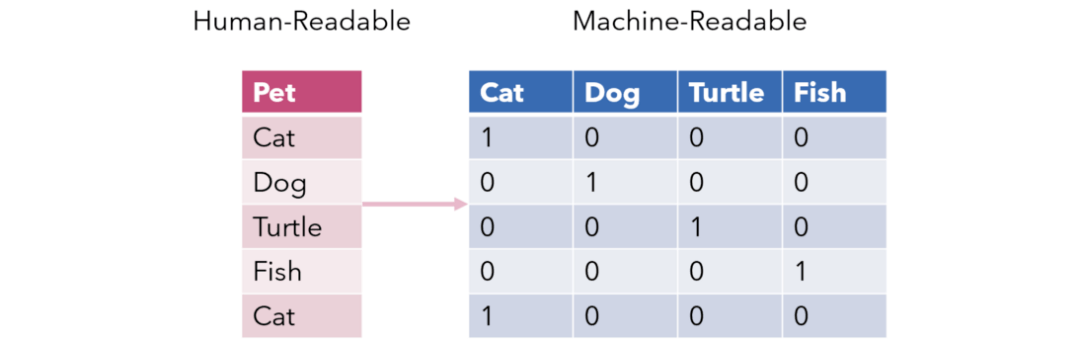
\includegraphics[width=0.6\linewidth]{one-hot-encoding.png}
        %\caption*{\footnotesize{The origin of the term ‘early-type’ lies with the original interpretation of the Hubble tuning fork diagram. This assumed that galaxies evolved from the left (early-type ellipticals) to the right (late-type spirals) in a sequence.
        %}}
        %\label{fig:fastdata}
    \end{figure}
    {\setlength\abovedisplayskip{0.1cm}
    \setlength\belowdisplayskip{0.1cm}
    \begin{equation}\label{equ:cross_entropy}
        \begin{split}
            H(\mathbf{y}, h_{\mathbf{\theta}}(\mathbf{x})) &= -\log P(y_{l(\mathbf{x}))} = 1|\mathbf{x})\\
            &= -\log p_{l(\mathbf{x}))}(\mathbf{x}))
        \end{split}
    \end{equation}
    }

\end{frame}

\begin{frame}
    \vspace{-0.1cm}
    {\noindent\large\textbf{损失函数与目标函数}}
    \vspace{0.4cm}

    {\setlength\abovedisplayskip{0.1cm}
        \setlength\belowdisplayskip{0.1cm}
        \begin{equation}\label{equ:cross_entropy}
            \begin{split}
                H(\mathbf{y}, h_{\mathbf{\theta}}(\mathbf{x})) &= -\log P(y_{l(\mathbf{x})}=1)|\mathbf{x})\\
                &= -\log p_{l(\mathbf{x}))}(\mathbf{x}))
            \end{split}
        \end{equation}
    }

    \begin{equation}\label{equ:cross_entropysimplized}
        E = -\sum\limits_{\mathbf{x} \in \Omega} log(p_{l(\mathbf{x}))}(\mathbf{x})))
    \end{equation}

    \begin{equation}\label{equ:unetobj}
        E = -\sum\limits_{\mathbf{x} \in \Omega} w(\mathbf{x}) log(p_{l(\mathbf{x}))}(\mathbf{x})))
    \end{equation}
\end{frame}


\begin{frame}
    \vspace{-0.1cm}
    {\noindent\large\textbf{权重函数}}
    \vspace{0.4cm}



    %\begin{figure}
    %   \vspace{-0.2cm}  %调整图片与上文的垂直距离
    %   \setlength{\belowcaptionskip}{-0.4cm}   %调整图片标题与下文距离
    %   \setlength{\abovecaptionskip}{0.4cm}   %调整图片标题与下文距离
    %  \centering%
    %    \hspace{0.05cm}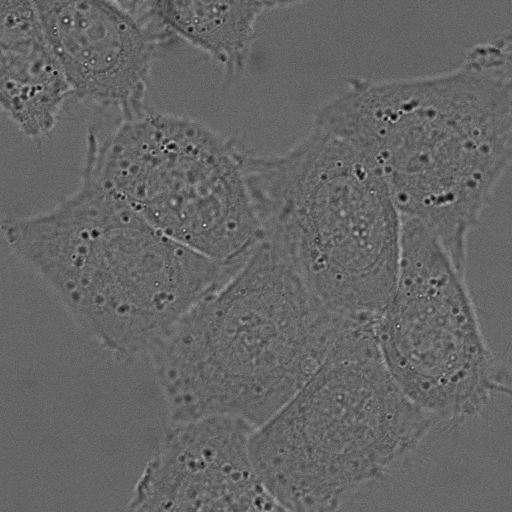
\includegraphics[width=0.2\linewidth]{DIC-C2DH-HeLa-02-t038.png}
    %    \hspace{0.05cm}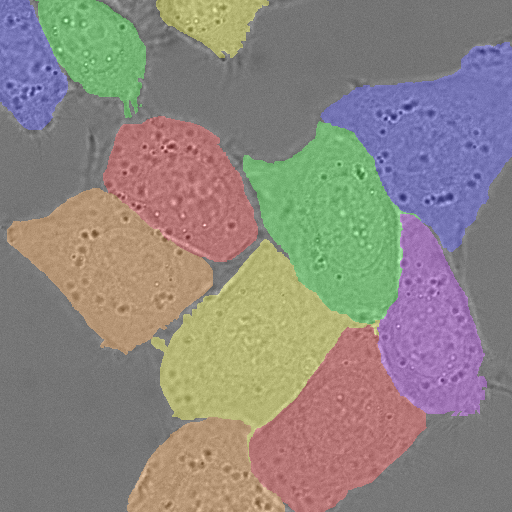
\includegraphics[width=0.2\linewidth]{DIC-C2DH-HeLa-02-t038-overlay.png}\\
    %    \hspace{0.05cm}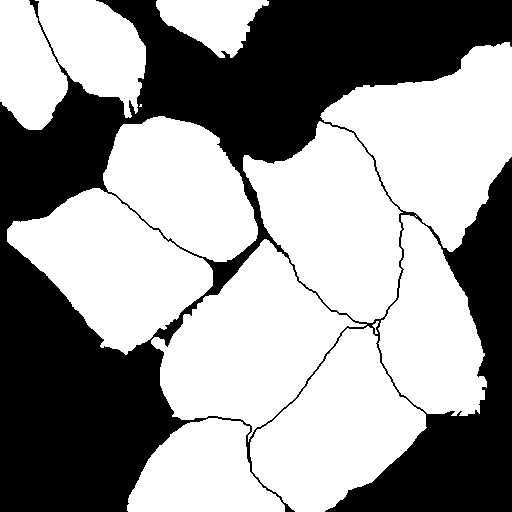
\includegraphics[width=0.2\linewidth]{DIC-C2DH-HeLa-02-t038-mask.png}
    %    \hspace{0.05cm}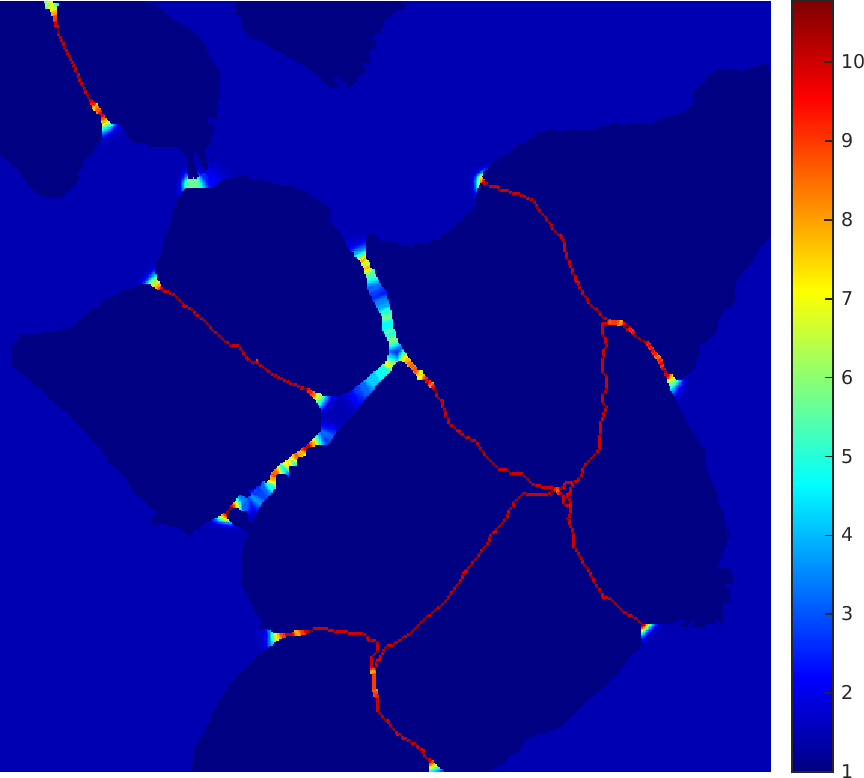
\includegraphics[width=0.2\linewidth]{weightmap.png}
    %\caption*{\footnotesize{
    %用DIC(差分干涉对比度)显微镜记录玻璃上的HeLa细胞。(a)原始图像。(b)参考分割结果。不同的颜色表示HeLa细胞的不同实例。(c)生成的分割掩码(白色:前景,黑色:背景)。(d)像素级的损失权重,以促使网络模型更好地学习识别边界像素。图像数据来自文献\citet{Unet2015Olaf}
    %%HeLa cells on glass recorded with DIC (differential interference contrast) microscopy. (a) raw image. (b) overlay with ground truth segmentation. Different colors indicate different instances of the HeLa cells. (c) generated segmentation mask (white: foreground, black: background). (d) map with a pixel-wise loss weight to force the network to learn the border pixels.
    %}}
    %\label{fig:fastdata}
    %\end{figure}

    \begin{columns}
        \vspace{-0.5cm}
        \begin{column}{0.6\linewidth}

            \begin{figure}
                \vspace{-0.2cm}  %调整图片与上文的垂直距离
                \setlength{\belowcaptionskip}{-0.4cm}   %调整图片标题与下文距离
                \setlength{\abovecaptionskip}{0.4cm}   %调整图片标题与下文距离
                \centering%
                \hspace{0.05cm}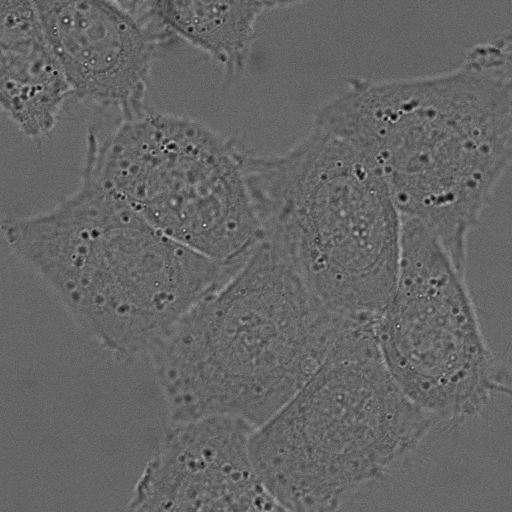
\includegraphics[width=0.34\linewidth]{DIC-C2DH-HeLa-02-t038.png}
                \hspace{0.05cm}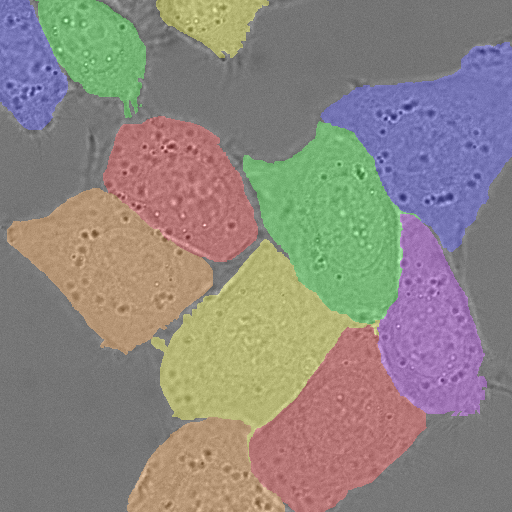
\includegraphics[width=0.34\linewidth]{DIC-C2DH-HeLa-02-t038-overlay.png}\\
                \hspace{0.05cm}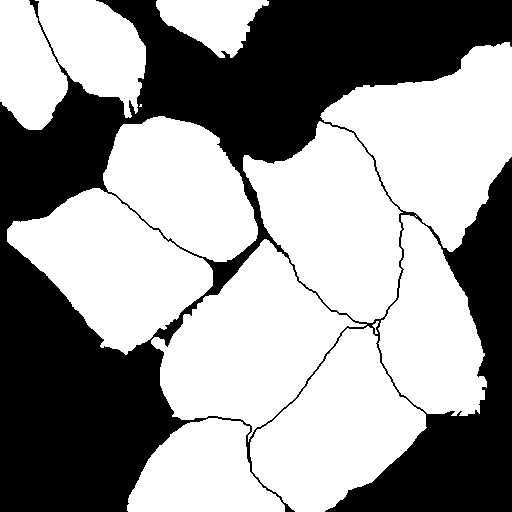
\includegraphics[width=0.34\linewidth]{DIC-C2DH-HeLa-02-t038-mask.png}
                \hspace{0.05cm}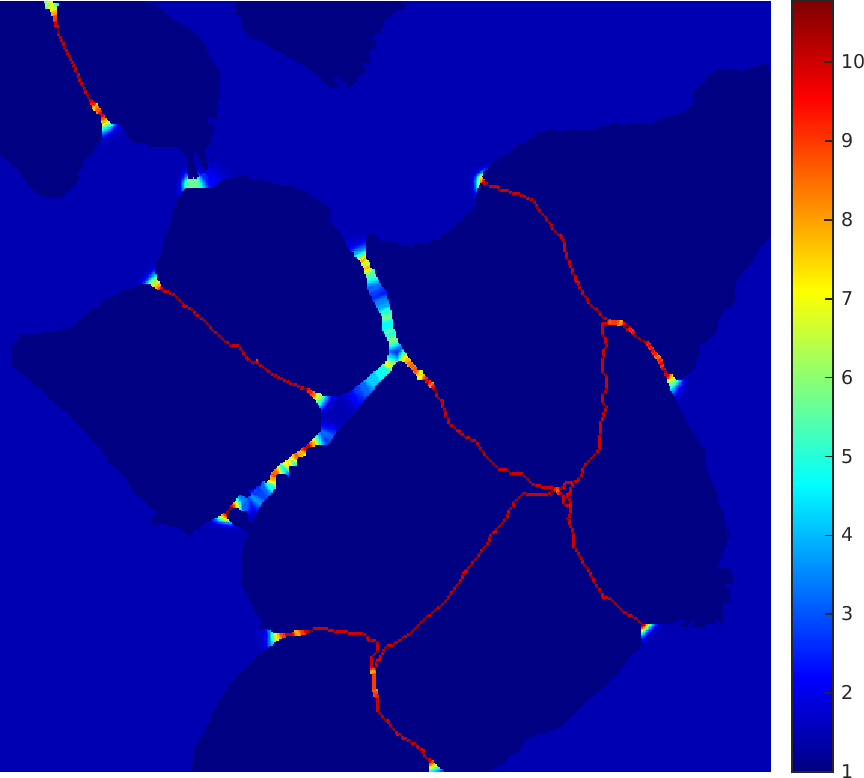
\includegraphics[width=0.34\linewidth]{weightmap.png}
                %\caption*{\footnotesize{用DIC(差分干涉对比度)显微镜记录玻璃上的HeLa细胞。(a)原始图像。(b)参考分割结果。不同的颜色表示HeLa细胞的不同实例。(c)生成的分割掩码(白色:前景,黑色:背景)。(d)像素级的损失权重,以促使网络模型更好地学习识别边界像素。图像数据来自文献\citet{Unet2015Olaf}
                %HeLa cells on glass recorded with DIC (differential interference contrast) microscopy. (a) raw image. (b) overlay with ground truth segmentation. Different colors indicate different instances of the HeLa cells. (c) generated segmentation mask (white: foreground, black: background). (d) map with a pixel-wise loss weight to force the network to learn the border pixels.
                %}}
                \label{fig:fastdata}
            \end{figure}

        \end{column}

        \begin{column}{0.4\linewidth}
            \footnotesize
            用DIC(差分干涉对比度)显微镜记录玻璃上的HeLa细胞。(a)原始图像。(b)参考分割结果。不同的颜色表示HeLa细胞的不同实例。(c)生成的分割掩码(白色:前景,黑色:背景)。(d)像素级的损失权重,以促使网络模型更好地学习识别边界像素。图像数据来自文献\citet{Unet2015Olaf}
        \end{column}
    \end{columns}


    {\setlength\abovedisplayskip{0.1cm}
    \setlength\belowdisplayskip{0.1cm}
    \begin{equation}\label{equ:weights}
        w(\mathbf{x}) = w_c(\mathbf{x}) + w_0 \cdot exp(-\frac{ (d_1 (\mathbf{x}) + d_2(\mathbf{x}) )^2  }{2\sigma^2})
    \end{equation}
    }
    $d_1$和$d_2$分别表示一个像素距离最近和第二近细胞的边界的距离。


\end{frame}




\section{数据预处理与数据增强}
\begin{frame}[allowframebreaks]
    \frametitle{\textsc{目录}} \vspace{-0.3cm}
    \begin{spacing}{0.0}
        \tableofcontents[currentsection,hideallsubsections]
    \end{spacing}   % 若不想要目录, 注释掉该句
\end{frame}

\begin{frame}
    %\vspace{-0.1cm}
    %{\noindent\large\textbf{数据增强}}
    %\vspace{0.4cm}



    %\begin{figure}
    %   \vspace{-0.2cm}  %调整图片与上文的垂直距离
    %   \setlength{\belowcaptionskip}{-0.4cm}   %调整图片标题与下文距离
    %   \setlength{\abovecaptionskip}{0.4cm}   %调整图片标题与下文距离
    %  \centering%
    %    \hspace{0.05cm}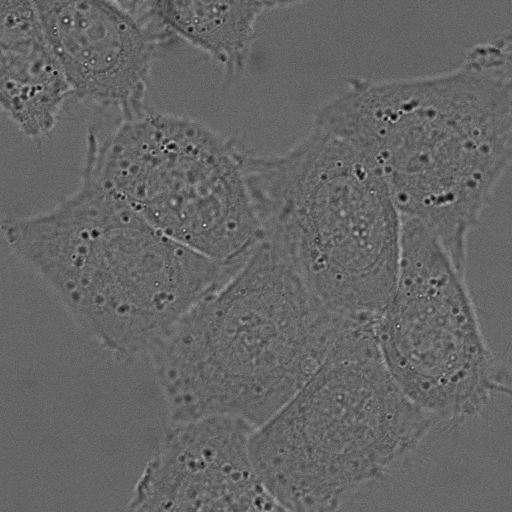
\includegraphics[width=0.2\linewidth]{DIC-C2DH-HeLa-02-t038.png}
    %    \hspace{0.05cm}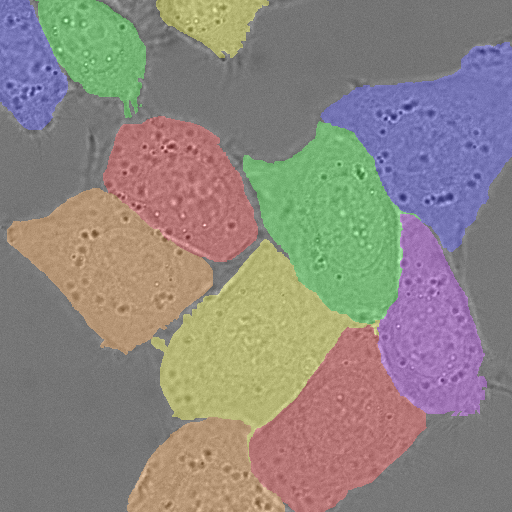
\includegraphics[width=0.2\linewidth]{DIC-C2DH-HeLa-02-t038-overlay.png}\\
    %    \hspace{0.05cm}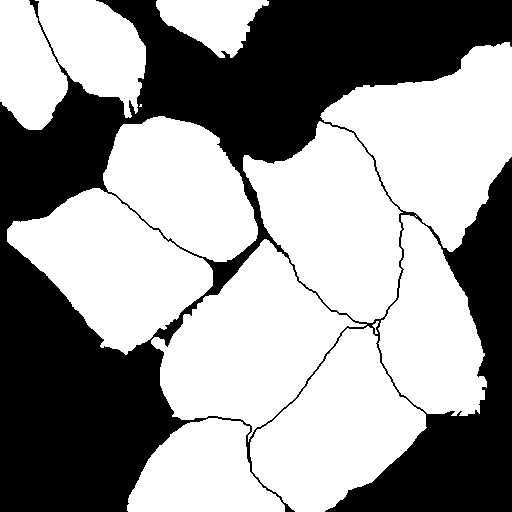
\includegraphics[width=0.2\linewidth]{DIC-C2DH-HeLa-02-t038-mask.png}
    %    \hspace{0.05cm}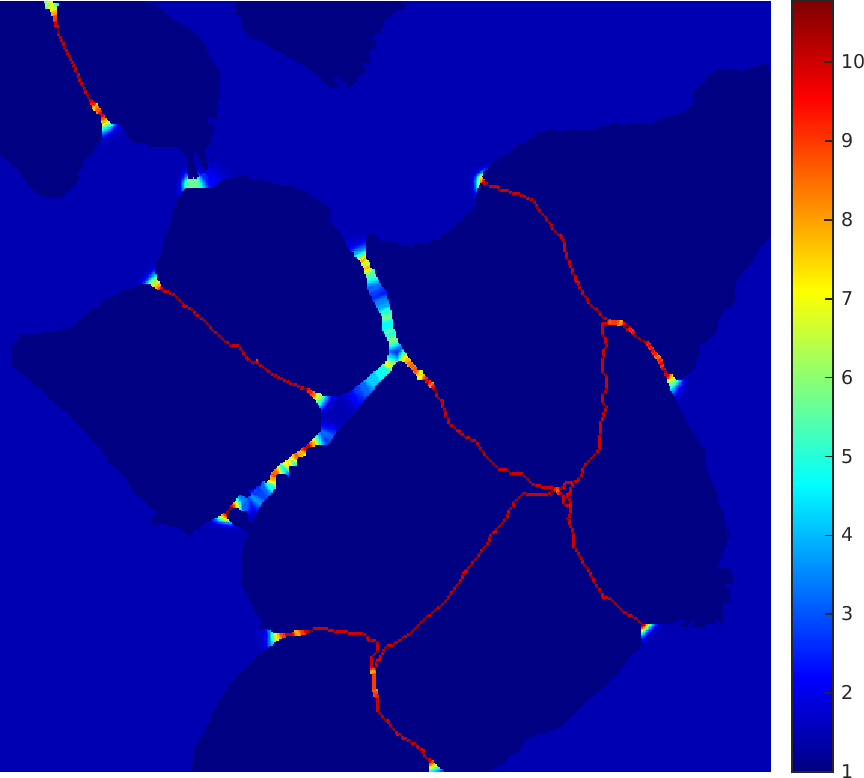
\includegraphics[width=0.2\linewidth]{weightmap.png}
    %\caption*{\footnotesize{
    %用DIC(差分干涉对比度)显微镜记录玻璃上的HeLa细胞。(a)原始图像。(b)参考分割结果。不同的颜色表示HeLa细胞的不同实例。(c)生成的分割掩码(白色:前景,黑色:背景)。(d)像素级的损失权重,以促使网络模型更好地学习识别边界像素。图像数据来自文献\citet{Unet2015Olaf}
    %%HeLa cells on glass recorded with DIC (differential interference contrast) microscopy. (a) raw image. (b) overlay with ground truth segmentation. Different colors indicate different instances of the HeLa cells. (c) generated segmentation mask (white: foreground, black: background). (d) map with a pixel-wise loss weight to force the network to learn the border pixels.
    %}}
    %\label{fig:fastdata}
    %\end{figure}

    \begin{columns}
        \vspace{-0.5cm}
        \begin{column}{0.6\linewidth}

            \begin{figure}
                \vspace{-0.2cm}  %调整图片与上文的垂直距离
                \setlength{\belowcaptionskip}{-0.4cm}   %调整图片标题与下文距离
                \setlength{\abovecaptionskip}{0.4cm}   %调整图片标题与下文距离
                \centering%
                \hspace{0.05cm}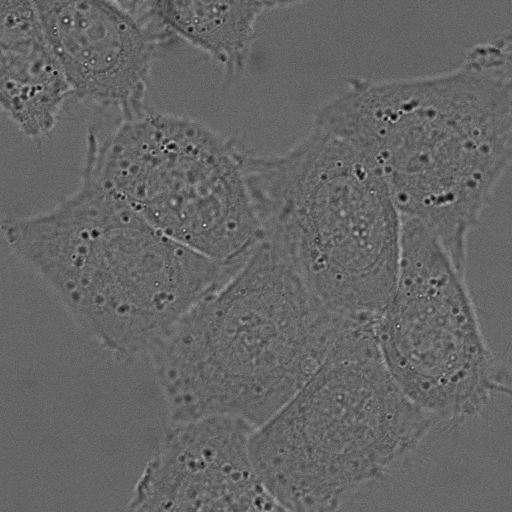
\includegraphics[width=0.34\linewidth]{DIC-C2DH-HeLa-02-t038.png}
                \hspace{0.05cm}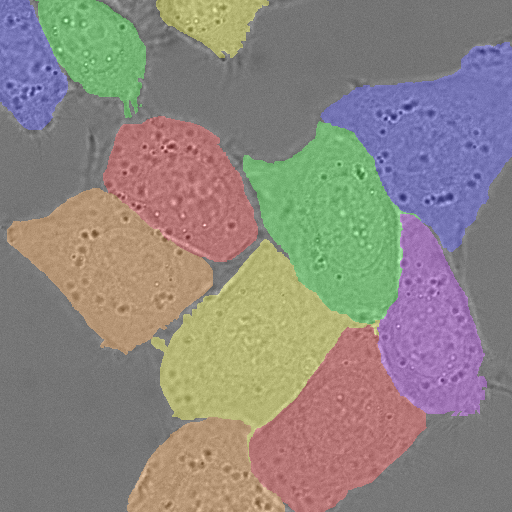
\includegraphics[width=0.34\linewidth]{DIC-C2DH-HeLa-02-t038-overlay.png}\\
                \hspace{0.05cm}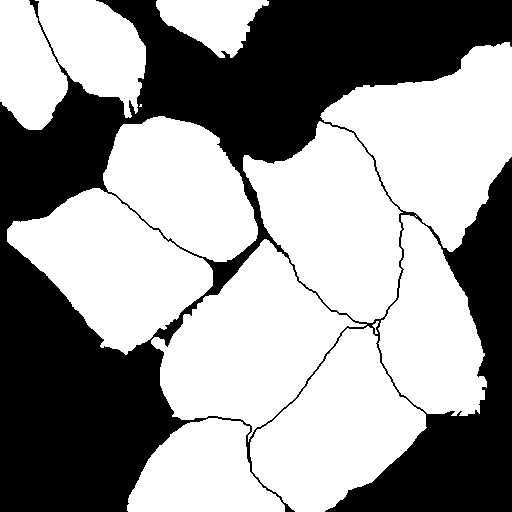
\includegraphics[width=0.34\linewidth]{DIC-C2DH-HeLa-02-t038-mask.png}
                \hspace{0.05cm}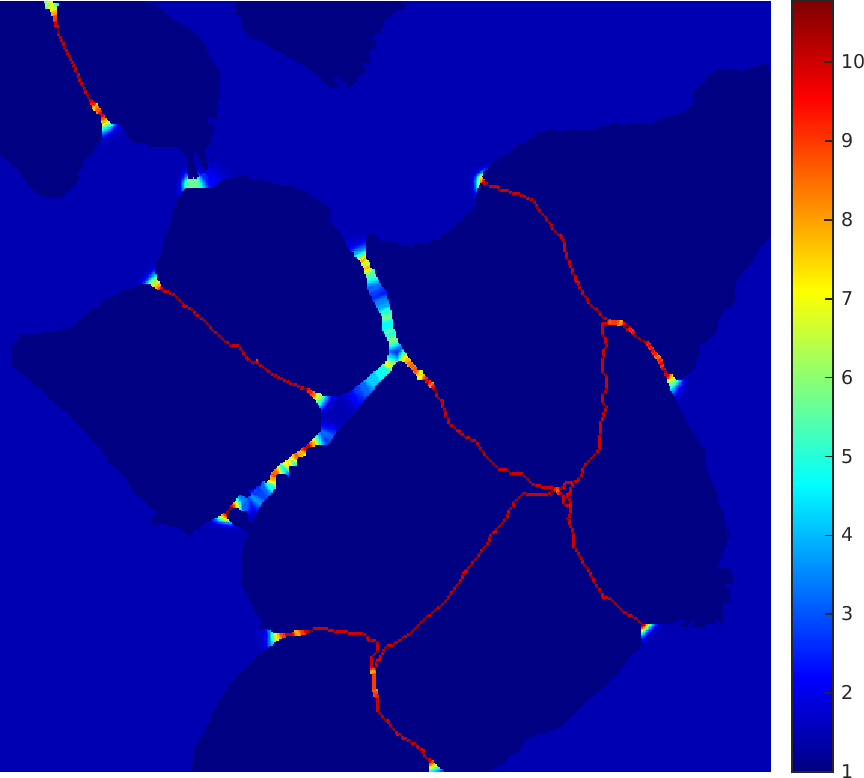
\includegraphics[width=0.34\linewidth]{weightmap.png}
                %\caption*{\footnotesize{用DIC(差分干涉对比度)显微镜记录玻璃上的HeLa细胞。(a)原始图像。(b)参考分割结果。不同的颜色表示HeLa细胞的不同实例。(c)生成的分割掩码(白色:前景,黑色:背景)。(d)像素级的损失权重,以促使网络模型更好地学习识别边界像素。图像数据来自文献\citet{Unet2015Olaf}
                %HeLa cells on glass recorded with DIC (differential interference contrast) microscopy. (a) raw image. (b) overlay with ground truth segmentation. Different colors indicate different instances of the HeLa cells. (c) generated segmentation mask (white: foreground, black: background). (d) map with a pixel-wise loss weight to force the network to learn the border pixels.
                %}}
                \label{fig:fastdata}
            \end{figure}

        \end{column}

        \begin{column}{0.4\linewidth}
            \footnotesize
            用DIC(差分干涉对比度)显微镜记录玻璃上的HeLa细胞。(a)原始图像。(b)参考分割结果。不同的颜色表示HeLa细胞的不同实例。(c)生成的分割掩码(白色:前景,黑色:背景)。(d)像素级的损失权重,以促使网络模型更好地学习识别边界像素。图像数据来自文献\citet{Unet2015Olaf}
        \end{column}
    \end{columns}

    \vspace{0.2cm}

    数据量与经验\\
    平移、旋转、形态


\end{frame}


\begin{frame}
    %\vspace{-0.1cm}
    %{\noindent\large\textbf{数据增强}}
    %\vspace{0.4cm}


    %\begin{columns}
    %\vspace{-0.5cm}
    %	\begin{column}{0.6\linewidth}
    %
    %
    %\end{figure}
    %
    %	\end{column}
    %
    %	\begin{column}{0.4\linewidth}
    %   \footnotesize
    %			用DIC(差分干涉对比度)显微镜记录玻璃上的HeLa细胞。(a)原始图像。(b)参考分割结果。不同的颜色表示HeLa细胞的不同实例。(c)生成的分割掩码(白色:前景,黑色:背景)。(d)像素级的损失权重,以促使网络模型更好地学习识别边界像素。图像数据来自文献\citet{Unet2015Olaf}
    %	\end{column}
    %\end{columns}

    \begin{figure}
        \vspace{-0.2cm}  %调整图片与上文的垂直距离
        \setlength{\belowcaptionskip}{-0.4cm}   %调整图片标题与下文距离
        \setlength{\abovecaptionskip}{0.4cm}   %调整图片标题与下文距离
        \centering%
        \hspace{0.05cm}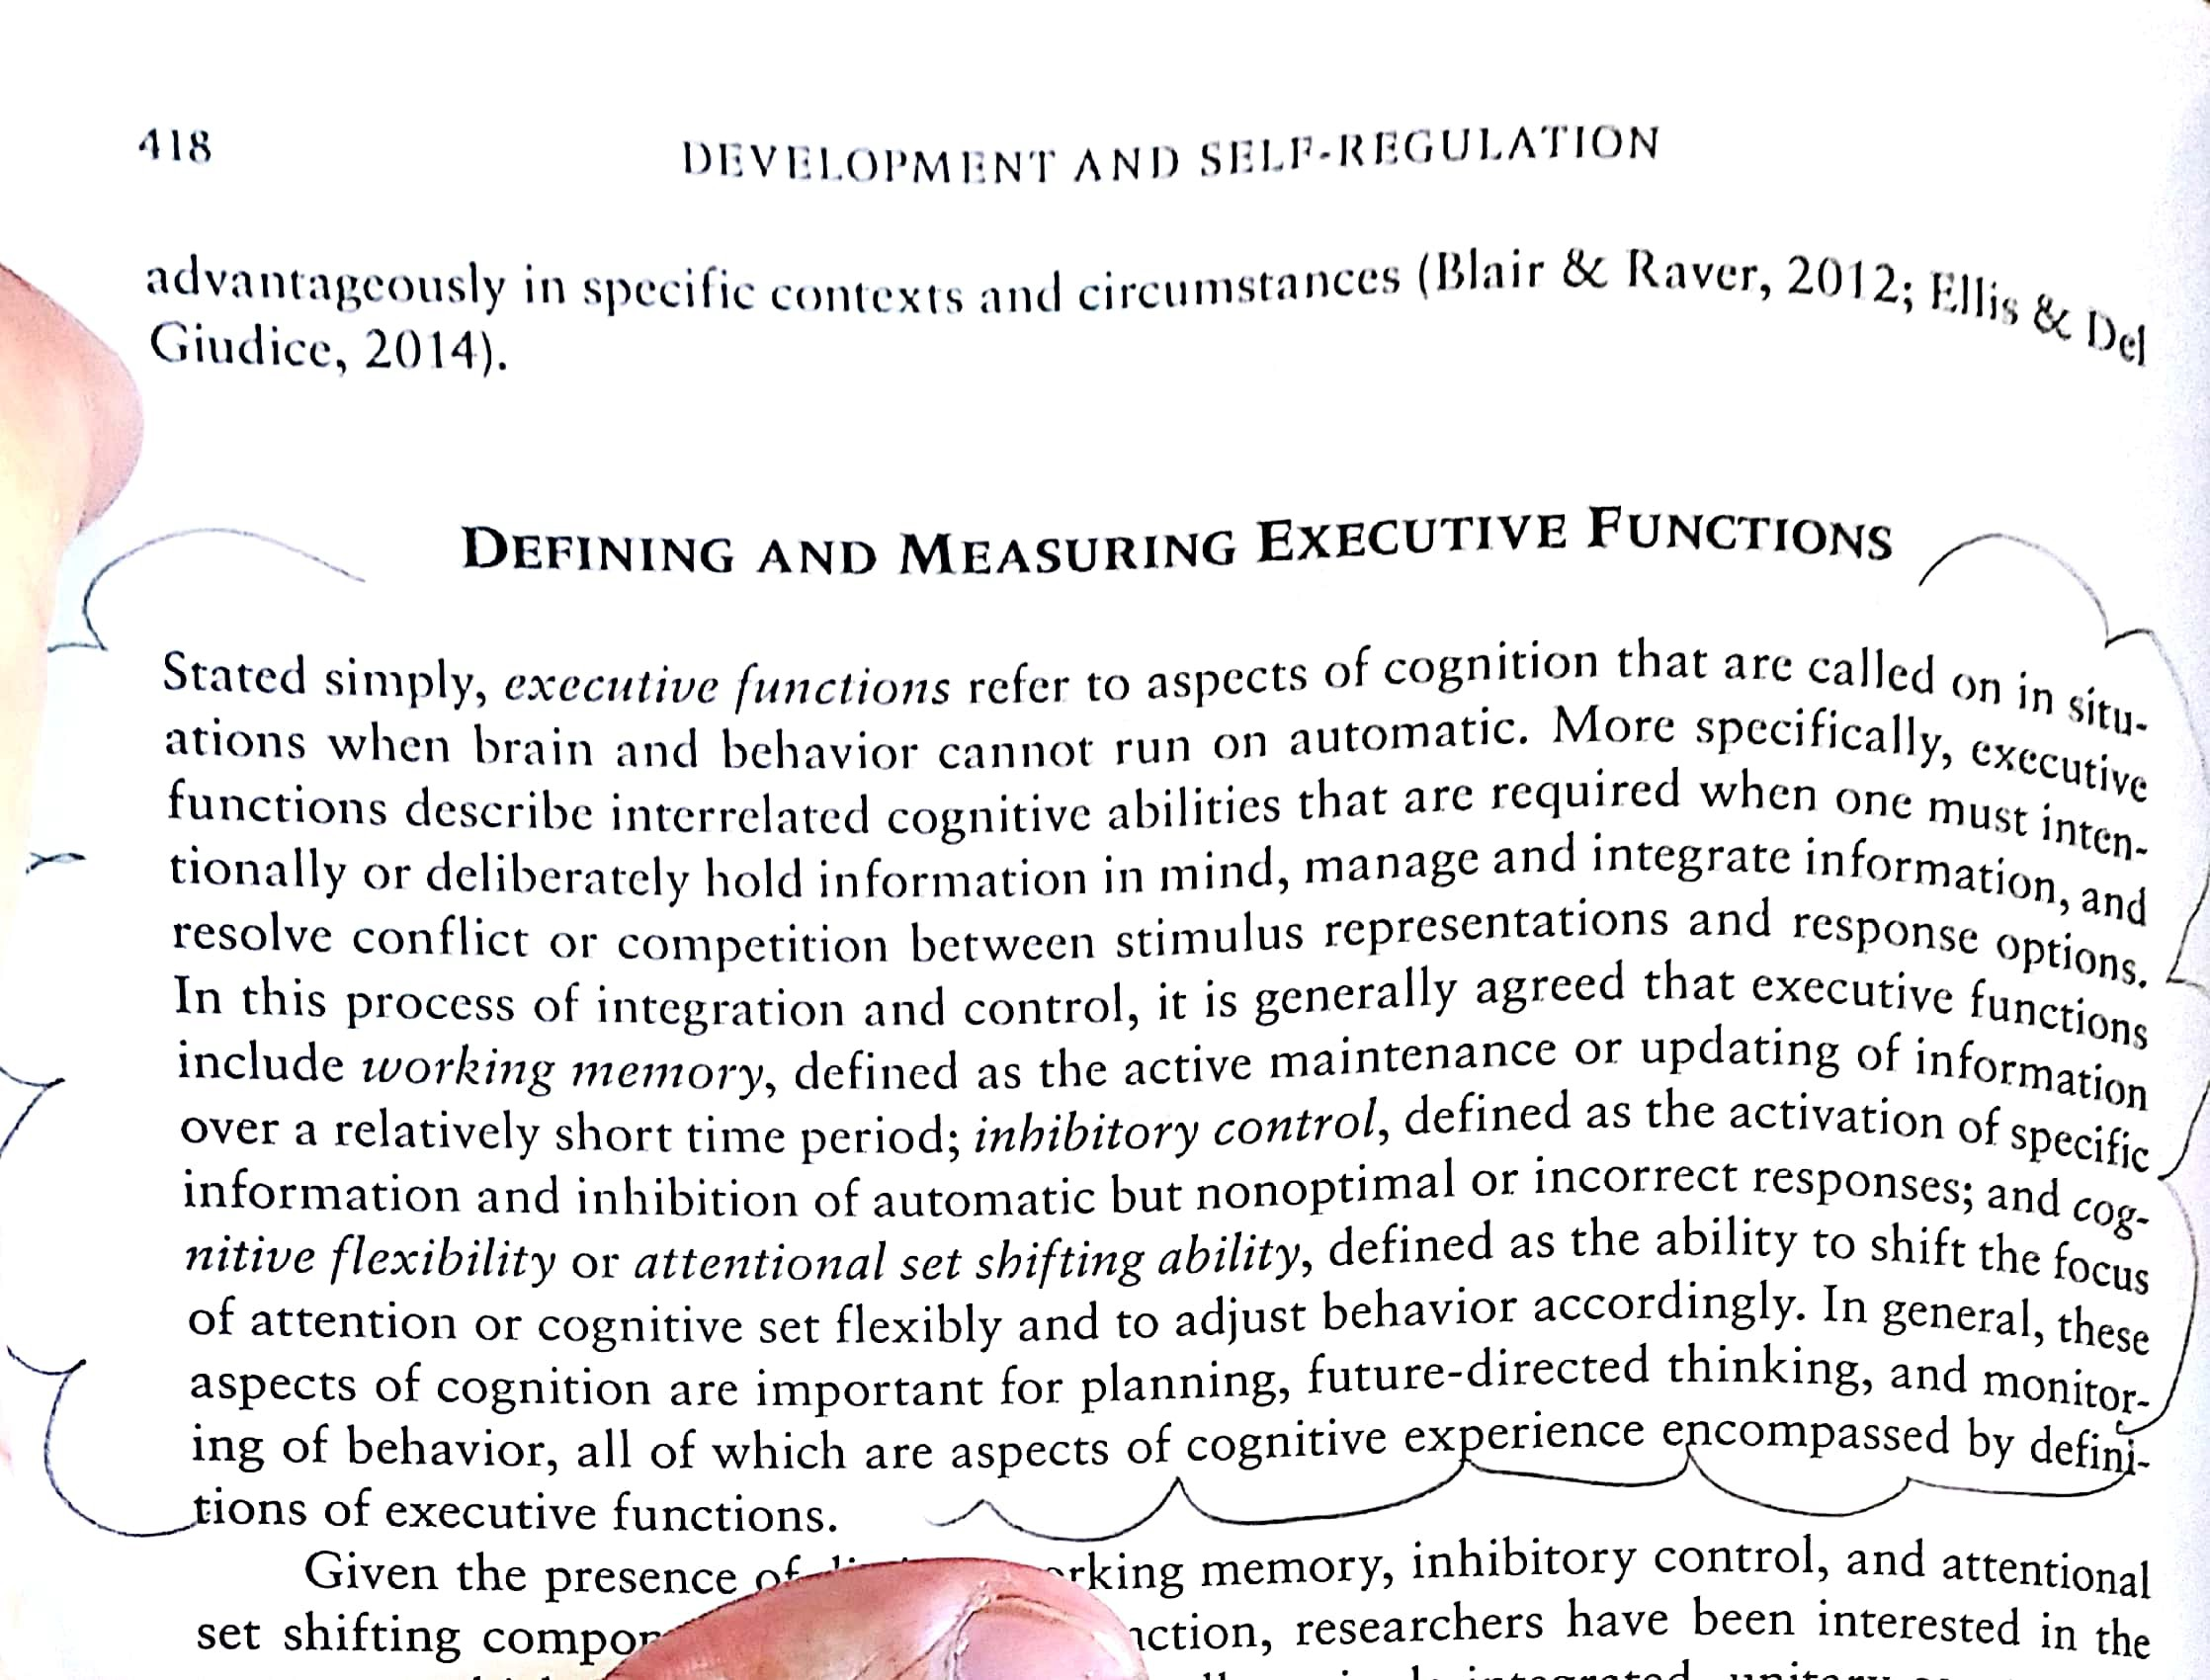
\includegraphics[width=0.8\linewidth]{Distortions.jpg}\\
        %\hspace{0.05cm}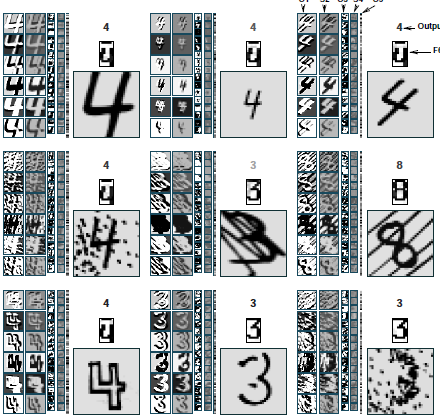
\includegraphics[width=0.34\linewidth]{UnusualDistortionNoises.png}%\\
        %\caption*{\footnotesize{用DIC(差分干涉对比度)显微镜记录玻璃上的HeLa细胞。(a)原始图像。(b)参考分割结果。不同的颜色表示HeLa细胞的不同实例。(c)生成的分割掩码(白色:前景,黑色:背景)。(d)像素级的损失权重,以促使网络模型更好地学习识别边界像素。图像数据来自文献\citet{Unet2015Olaf}
        %HeLa cells on glass recorded with DIC (differential interference contrast) microscopy. (a) raw image. (b) overlay with ground truth segmentation. Different colors indicate different instances of the HeLa cells. (c) generated segmentation mask (white: foreground, black: background). (d) map with a pixel-wise loss weight to force the network to learn the border pixels.
        %}}
        \label{fig:fastdata}
    \end{figure}

    \vspace{0.2cm}

    数据量与经验\\
    平移、旋转、形态


\end{frame}


\begin{frame}
    %\vspace{-0.1cm}
    %{\noindent\large\textbf{数据增强}}
    %\vspace{0.4cm}


    %\begin{columns}
    %\vspace{-0.5cm}
    %	\begin{column}{0.6\linewidth}
    %
    %
    %\end{figure}
    %
    %	\end{column}
    %
    %	\begin{column}{0.4\linewidth}
    %   \footnotesize
    %			用DIC(差分干涉对比度)显微镜记录玻璃上的HeLa细胞。(a)原始图像。(b)参考分割结果。不同的颜色表示HeLa细胞的不同实例。(c)生成的分割掩码(白色:前景,黑色:背景)。(d)像素级的损失权重,以促使网络模型更好地学习识别边界像素。图像数据来自文献\citet{Unet2015Olaf}
    %	\end{column}
    %\end{columns}

    \begin{figure}
        \vspace{-0.2cm}  %调整图片与上文的垂直距离
        \setlength{\belowcaptionskip}{-0.4cm}   %调整图片标题与下文距离
        \setlength{\abovecaptionskip}{0.4cm}   %调整图片标题与下文距离
        \centering%
        %\hspace{0.05cm}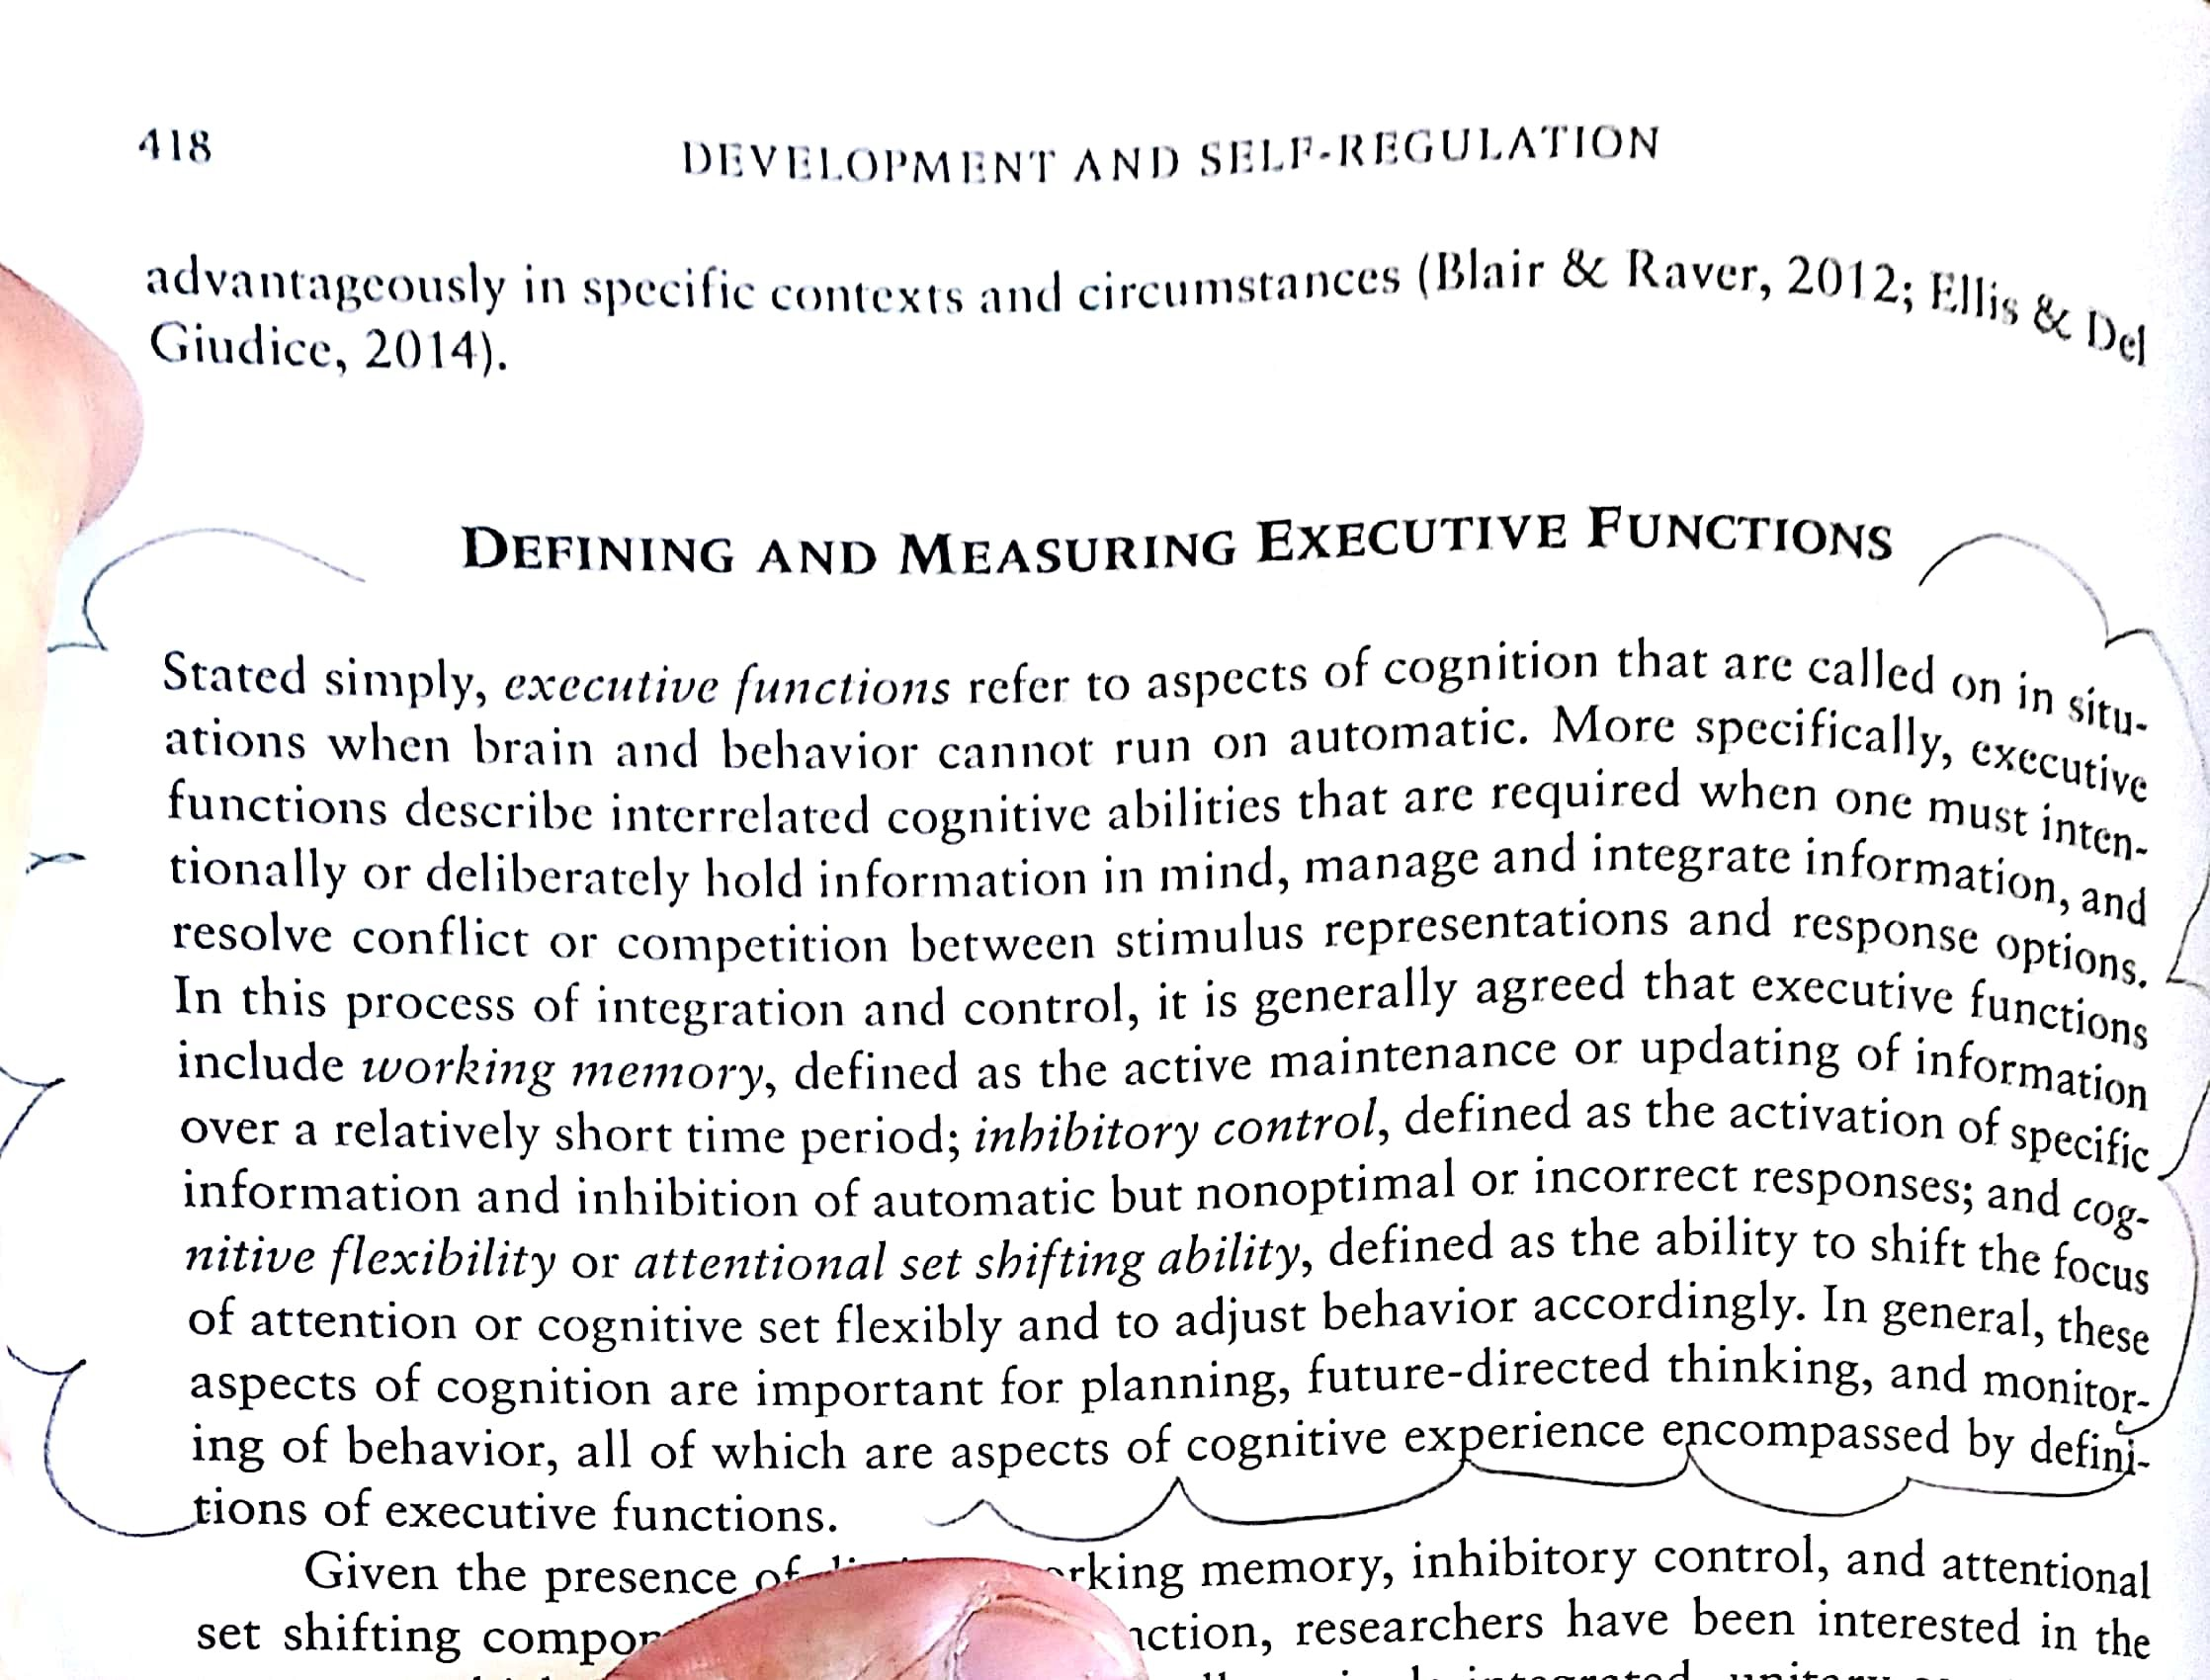
\includegraphics[width=0.34\linewidth]{Distortions.jpg}\\
        \hspace{0.05cm}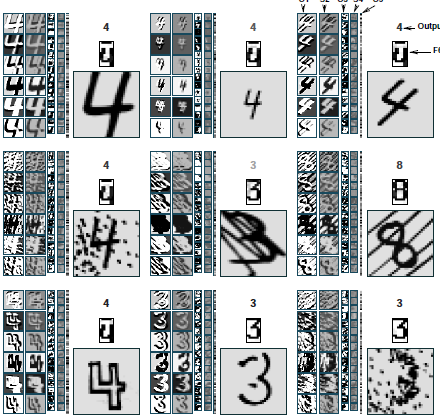
\includegraphics[width=0.7\linewidth]{UnusualDistortionNoises.png}%\\
        %\caption*{\footnotesize{用DIC(差分干涉对比度)显微镜记录玻璃上的HeLa细胞。(a)原始图像。(b)参考分割结果。不同的颜色表示HeLa细胞的不同实例。(c)生成的分割掩码(白色:前景,黑色:背景)。(d)像素级的损失权重,以促使网络模型更好地学习识别边界像素。图像数据来自文献\citet{Unet2015Olaf}
        %HeLa cells on glass recorded with DIC (differential interference contrast) microscopy. (a) raw image. (b) overlay with ground truth segmentation. Different colors indicate different instances of the HeLa cells. (c) generated segmentation mask (white: foreground, black: background). (d) map with a pixel-wise loss weight to force the network to learn the border pixels.
        %}}
        \label{fig:fastdata}
    \end{figure}

    \vspace{0.2cm}

    数据量与经验\\
    平移、旋转、形态


\end{frame}




\section{探讨与扩展阅读}
\begin{frame}[allowframebreaks]
    \frametitle{\textsc{目录}} \vspace{-0.3cm}
    \begin{spacing}{0.0}
        \tableofcontents[currentsection,hideallsubsections]
    \end{spacing}   % 若不想要目录, 注释掉该句
\end{frame}


\begin{frame}[allowframebreaks]
    \vspace{-0.1cm}
    {\noindent\large\textbf{探讨与扩展阅读}}
    \vspace{0.4cm}
    %\tiny
    \begin{itemize}
        \item[*] U-Net: Convolutional Networks for Biomedical Image Segmentation \citep{Unet2015Olaf}
        \item[*] nnU-Net: a self-configuring method for deep learning-based biomedical image segmentation \citep{Isensee2021NM}
        \item[*] nnU-Net: Self-adapting Framework for U-Net-Based Medical Image Segmentation \citep{Isensee2019}.
    \end{itemize}
\end{frame}




\section{思考题}
\begin{frame}[allowframebreaks]
    \frametitle{\textsc{目录}} \vspace{-0.3cm}
    \begin{spacing}{0.0}
        \tableofcontents[currentsection,hideallsubsections]
    \end{spacing}   % 若不想要目录, 注释掉该句
\end{frame}


\begin{frame}[allowframebreaks]
    \vspace{-0.1cm}
    {\noindent\large\textbf{思考题(选做)}}
    \vspace{0.4cm}
    \begin{itemize}
        \item[9.1] 请参考文献\citet{Unet2015Olaf}和网上调研,在课程提供的U-Net参考代码基础上添加数据增强模块,并测试和撰写简要说明。
        \item[9.2] 请尝试在课程提供的U-Net参考代码基础上添加公式(\ref{equ:weights})中的权重, 并测试和撰写简要说明。
    \end{itemize}
\end{frame}







\section{Reference}

\begin{frame}[allowframebreaks]{参考文献}
    \vspace{-0.3cm}
    \scriptsize%\tiny\scriptsize\footnotesize\small\normalsize\large\Large\LARGE\huge\Huge
    \normalem
    \bibliographystyle{apalike}%{mnras}
    \bibliography{example} % if your bibtex file is called example.bib
\end{frame}


\end{document}
